
\section{Penalty functions}

The employment of penalty functions is a paradigm for solving constrained optimisation problems. The central idea of this paradigm is to convert the constrained optimisation problem into an unconstrained optimisation problem that is augmented with a \emph{penalty function}, which penalises violations of the original constraints. The role of the penalty function is to allow steering the search towards feasible solutions in the search for optimal solutions. 

Consider the problem $(P): \mini\braces{f(x) : g(x) \leq 0, h(x) = 0, x \in X}$. A \emph{penalised version} of $P$ is given by 
$$
(P_\mu) : \mini\braces{f(x) + \mu\alpha(x) : x \in X},
$$
where $\mu > 0$ is a \emph{penalty term} and $\alpha(x) : \reals^n \mapsto \reals$ is a \emph{penalty function} of the form
%
\begin{equation} 
	\alpha(x) = \sum_{i=1}^m \phi(g_i(x)) + \sum_{i=1}^l\psi(h_i(x)). \label{eq:penalty_function}	
\end{equation}

For $\alpha(x)$ to be a suitable penalty function, one must observe that $\phi : \reals^n \mapsto \reals$ and $\psi: \reals^n \mapsto \reals$ are continuous and satisfy
%
\begin{align*}
	& \phi(y) \hspace{1.0pt}= 0 \text{ if } y \leq 0 \text{ and } \phi(y) \hspace{0.5pt}> 0 \text{ if } y > 0\\
	& \psi(y) = 0 \text{ if } y = 0 \text{ and } \psi(y) > 0 \text{ if } y \neq 0.
\end{align*}
%
Typical options are $\phi(y) = ([y]^+)^p$ with $p \in \integers_+$ and $\psi(y) = |y|^p$ with $p=1$ or $p=2$.

Figure \ref{ex1} illustrates the solution of $(P) : \mini\braces{x_1^2 + x_2^2 : x_1 + x_2 = 1, x \in \reals^2}$ using a penalty-based approach. Using $\alpha(x_1,x_2) = (x_1 + x_2 - 1)^2$, the penalised auxiliary problem $P_\mu$ becomes $(P_\mu) :\mini\braces{x_1^2 + x_2^2 + \mu(x_1 + x_2 - 1)^2 : x \in \reals^2}$. Since $f_{\mu}$ is convex and differentiable, necessary and sufficient optimality conditions $\nabla f_\mu(x) = 0$ imply:
%
\begin{align*}
& x_1 + \mu(x_1 + x_2 -1) = 0\\
& x_2 + \mu(x_1 + x_2- 1) = 0,
\end{align*}
which gives $x_1 = x_2 = \frac{\mu}{2\mu + 1}$. 

One can notice that, as $\mu$ increases, the solution of the unconstrained penalised problem, represented by the level curves, becomes closer to the optimal of the original constrained problem $P$, represented by the dot on the hyperplane defined by $x_1 + x_2 = 1$.

\begin{figure}[H]
	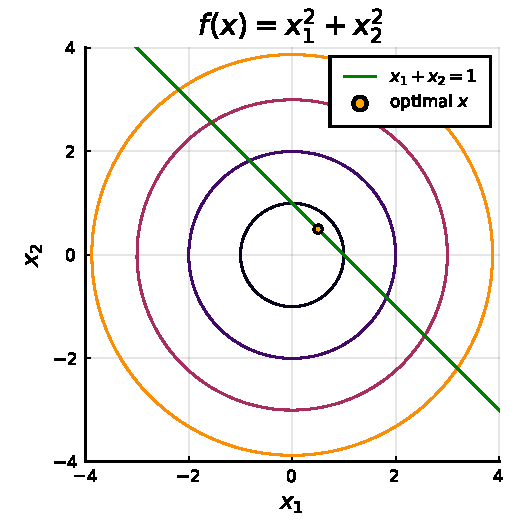
\includegraphics[width = 0.49\textwidth]{part_2/chapter_9/figures/ex1.pdf}
	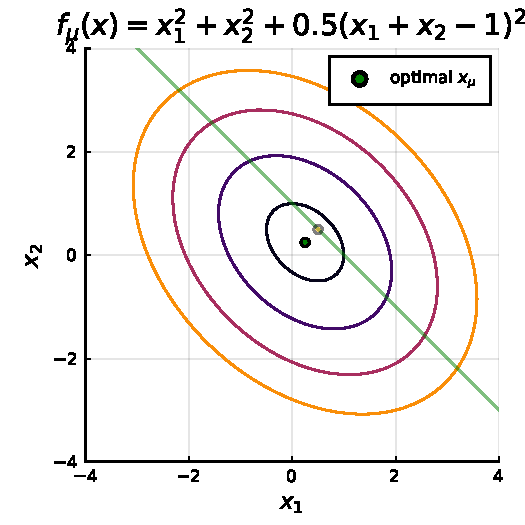
\includegraphics[width = 0.49\textwidth]{part_2/chapter_9/figures/ex2-1.pdf}
	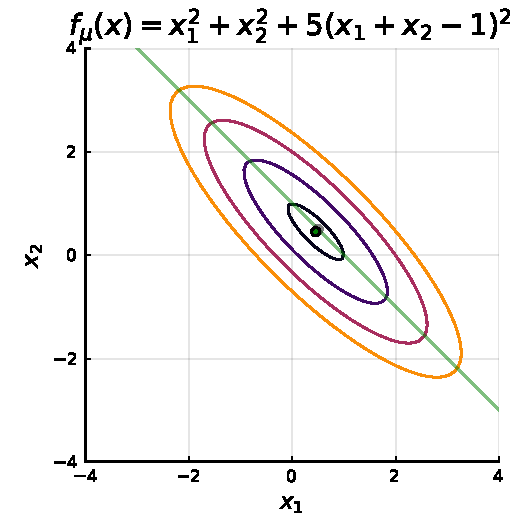
\includegraphics[width = 0.49\textwidth]{part_2/chapter_9/figures/ex2-3.pdf}
	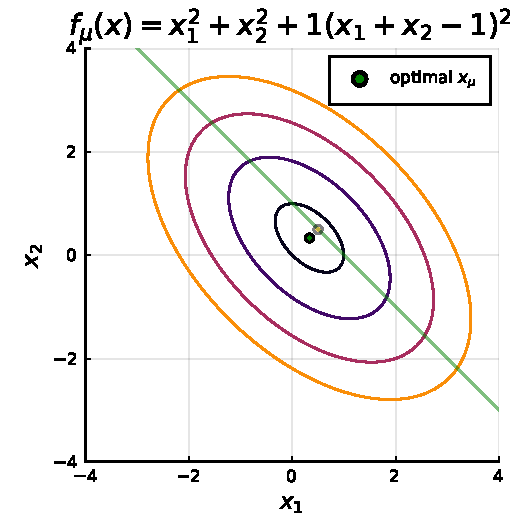
\includegraphics[width = 0.49\textwidth]{part_2/chapter_9/figures/ex2-2.pdf}
\caption{Solving the constrained problem $P$ (top left) by gradually increasing the penalty term $\mu$ (0.5, 1, and 5, in clockwise order)} \label{ex1}
\end{figure}


\subsection{Geometric interpretation}


A similar geometrical analysis to that performed with the Lagrangian duals can be employed for understanding how penalised problems can obtain optimal solutions. For that, let us the problem from the previous example $(P) : \mini\braces{x_1^2 + x_2^2 : x_1 + x_2 = 1, x \in \reals^2}$. Let $G: \reals^2 \rightarrow \reals^2$ be a mapping $\braces{[h(x), f(x)]: x \in \reals^2}$, and let $v(\epsilon) =$ $\mini\braces{x_1^2 + x_2^2 : x_1 + x_2 - 1 = \epsilon, \ x \in \reals^2}$. The optimal solution is $x_1 = $ $x_2 =$ $\frac{1+ \epsilon}{2}$ with $v(\epsilon) = \frac{(1+\epsilon)^2}{2}$. 

\begin{figure}
	\begin{tikzpicture}
		\node at (0,0) {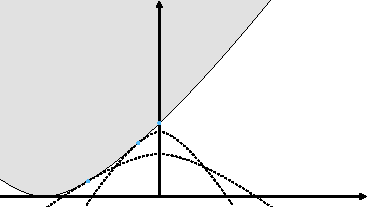
\includegraphics{part_2/chapter_9/figures/penalty_G.pdf}};
		\node at (-2.5,1.5) {$G$};
		\node[right] at (-0.5, 1.6) {\scriptsize $z = f(x)$};
		\node[left] at (3,-1.4) {\scriptsize $h(x) = \epsilon$}; 
		\node[right] at (1,1.3) {\scriptsize $v(\epsilon)$};
		\node[left] at (-0.4,-0.3) {\scriptsize $\epsilon_{\overline{\mu}}$};
		\node[left] at (-0.65,-0.55) {\scriptsize $\epsilon_{\mu_2}$};
		\node[left] at (-1.35,-1.1) {\scriptsize $\epsilon_{\mu_1}$};
		\node at (0.5,-1.9) {\scriptsize $f + \mu_2 h^2$};		
		\node at (2.4,-1.9) {\scriptsize $f + \mu_1 h^2$};
	\end{tikzpicture}
	\caption{Geometric representation of penalised problems in the mapping $G = [h(x), f(x)]$} \label{fig:Fig1}
\end{figure}

Minimising $f(x) + \mu(h(x)^2)$ consists of moving the curve downwards until a single contact point $\epsilon_\mu$ remains. One can notice that, as $\mu \rightarrow \infty$, $f + \mu h$ becomes sharper ($\mu_2 > \mu_1$), and $\epsilon_\mu$ \emph{converges} to the optimum $\epsilon_{\overline{\mu}}$. Figure \ref{fig:Fig1} illustrates this behaviour.

The shape of the penalised problem curve is due to the following. First, notice that
%
\begin{align*}
&\mini_x \braces{f(x) + \mu \sum_{i=1}^l(h_i(x))^2} \\
= & \mini_{x,\epsilon}\braces{f(x) + \mu ||\epsilon||^2 : h_i(x) = \epsilon, i = 1,\dots, l}\\
= & \mini_{\epsilon}\braces{ \mu||\epsilon||^2 + \mini_{x} \braces{f(x) : h_i(x) = \epsilon, i = 1, \dots, l}} \\
= & \mini_{\epsilon}\braces{\mu||\epsilon||^2 + v(\epsilon)}.
\end{align*}
%
Consider $l=1$, and let $x_\mu = \arg\min_x \braces{f(x) + \mu \sum_{i=1}^l(h_i(x))^2}$ with $h(x_\mu) = \epsilon_\mu$, implying that $\epsilon_\mu = \arg\min_{\epsilon}\braces{\mu||\epsilon||^2 + v(\epsilon)}$. Then, the following holds
\begin{enumerate}
\item $f(x_\mu) + \mu(h(x_\mu))^2 = \mu \epsilon_\mu^2 + v(\epsilon_\mu) \Rightarrow f(x_\mu) = v(\epsilon_\mu)$, since $h(x_\mu) = \epsilon_\mu$; 
\item and $v'(\epsilon_\mu) = \frac{\partial}{\partial \epsilon}(f(x_\mu) + \mu(h(x_\mu))^2 - \mu\epsilon_\mu^2) = -2\mu\epsilon_\mu$. 
\end{enumerate}

Therefore, $(h(x_\mu), f(x_\mu)) = (\epsilon_\mu, v(\epsilon_\mu))$. Denoting $f(x_\mu) + \mu h(x_\mu)^2 = k_\mu$, we see the parabolic function $f = k_\mu - \mu\epsilon^2$ matching $v(\epsilon_\mu)$ for $\epsilon=\epsilon_\mu$ and has the slope $-2\mu \epsilon$, matching that of $v(\epsilon)$ at that point.


\subsection{Penalty function methods}


The convergent behaviour of the penalised problem as the penalty term $\mu$ increases inspires the development of a simple yet powerful method for optimising constrained optimisation problems. 

That is, consider the problem $P$ defined as 
%
\begin{align*}
(P) : \mini 	   &f(x) \\
				   &g_i(x) \leq 0,  i = 1,\dots,m, \\
                   &h_i(x) = 0,  i = 1,\dots,l, \\
                   &x \in X.
\end{align*}
%
We seek to solve $P$ by solving $\sup_\mu \braces{\theta(\mu)}$ for $\mu > 0$, where
$$ 
\theta(\mu) = \mini \braces{f(x) + \mu\alpha(x) : x \in X} 
$$
and $\alpha(x)$ is a penalty function as defined in \eqref{eq:penalty_function}. For that to be possible, we need first to state a convergence result guaranteeing that 
$$ 
\mini\braces{f(x) : g(x) \leq 0, h(x) = 0, x \in X} = \sup_{\mu \geq 0} \theta(\mu) = \lim_{\mu \rightarrow\infty}\theta(\mu).
$$
In practice, that would mean that $\mu_k$ can be increased at each iteration $k$ until a suitable tolerance is achieved. Theorem \ref{thm:conv_pen_method} states the convergence of penalty based methods.

\begin{theorem}[Convergence of penalty-based methods]\label{thm:conv_pen_method}
Consider the problem $P$, where $f$, $g_i$ for $i=1,\dots,m$, and $h_i$ for $i=1,\dots,l$ are continuous, and $X \subset \reals^n$ a compact set. Suppose that, for each $\mu$, there exists $x_\mu = \arg\min \braces{f(x) + \alpha(x) : x \in X}$, where $\alpha$ is a suitable penalty function and $\braces{x_\mu}$ is contained within $X$. Then
$$ \min_x\braces{f(x) : g(x) \leq 0, h(x) = 0, x \in X} = \sup_{\mu \geq 0}\braces{\theta(\mu)} = \lim_{\mu \rightarrow\infty}\theta(\mu),
$$
where $\theta(\mu) = \min_x \braces{f(x) + \mu\alpha(x) : x \in X} = f(x_\mu) + \mu\alpha(x_\mu)$. Also, the limit of any convergent subsequence of $\braces{x_\mu}$ is optimal to the original problem and $\mu\alpha(x_\mu) \rightarrow 0$ as $\mu \rightarrow \infty$.
\end{theorem}
%
\begin{proof}
	We first show that $\theta(\mu)$ are nondecreasing function of $\mu$. Let $0 < \lambda < \mu$. From the definition of $\theta(\mu)$, we have that 
	%
	\begin{equation} 
		f(x_\mu) + \lambda\alpha(x_\mu) \geq f(x_\lambda) + \lambda \alpha(x_\lambda) \label{eq:part1}
	\end{equation}
	%
	Adding and subtracting $\mu\alpha(x_\mu)$ in the left side of \eqref{eq:part1}, we conclude that $\theta(\mu) \geq \theta(\lambda)$. Now, for $x \in X$ with $g(x) \leq 0$ and $h(x) = 0$, notice that $\alpha(x) = 0$. This implies that
	%
	\begin{equation} \label{eq:ge_side}
		 f(x) = f(x) + \mu\alpha(x) \geq \inf_x\braces{f(x) + \mu\alpha(x) : x \in X} = \theta(\mu)
	\end{equation}
	%
	and, therefore, $\theta(\mu)$ is bounded above, and thus $\sup_{\mu \geq 0}\theta(\mu) = \lim_{\mu \rightarrow\infty}\theta(\mu)$. For that to be the case, we must have that $\mu\alpha(x_\mu) \rightarrow 0$ as $\mu \rightarrow \infty$. Moreover, we notice from \eqref{eq:ge_side} that
	
	\begin{equation} \label{eq:ge_side2}
		 \min_x\braces{f(x) : g(x) \leq 0, h(x) = 0, x \in X} \geq \lim_{\mu \rightarrow\infty}\theta(\mu).
	\end{equation}
	
	On the other hand, take any convergent subsequence $\braces{x_{\mu_k}}$ of $\braces{x_\mu}_{\mu \rightarrow \infty}$ with limit $\overline{x}$. Then
	$$
	\sup_{\mu \geq 0} \theta(\mu) \geq \theta(\mu_k) = f(x_{\mu_k}) + \mu\alpha(x_{\mu_k}) \geq f(x_{\mu_k}).
	$$
	Since $x_{\mu_k} \rightarrow \overline{x}$ as $\mu \rightarrow \infty$ and $f$ is continuous, this implies that $\sup_{\mu \geq 0} \theta(\mu) \geq f(\overline{x})$. Combined with \eqref{eq:ge_side2}, we have that $f(\overline{x}) = \sup_{\mu \geq 0}\braces{\theta(\mu)}$ and thus the result follows.
\end{proof}

The proof starts by demonstrating the nonincreasing behaviour of penalty functions and nondecreasing behaviour of $\theta(\mu)$ to allow for convergence. By noticing that
$$ 
f(x_\mu) + \lambda\alpha(x_\mu) + \mu\alpha(x_\mu) - \mu\alpha(x_\mu)  = \theta(\mu) +(\lambda - \mu)\alpha(x_\mu) \geq f(x_\lambda) + \lambda \alpha(x_\lambda) = \theta(\lambda)
$$
and that $\lambda - \mu < 0$, we can infer that $\theta(\mu) \geq \theta(\lambda)$. It is also interesting to notice how the objective function $f(x)$ and infeasibility $\alpha(x)$ behave as we increase the penalty coefficient $\mu$. For that, notice that using the same trick in the proof for two distinct values $0 < \lambda < \mu$, we have

\begin{enumerate}
	\item $f(x_\mu) + \lambda\alpha(x_\mu) \geq f(x_\lambda) + \lambda \alpha(x_\lambda)$ 
	\item $f(x_\lambda) + \mu\alpha(x_\lambda) \geq f(x_\mu) + \mu \alpha(x_\mu)$.
\end{enumerate}

Notice that in 1, we use the fact that $x_\lambda = \arg\min_x \theta(\lambda) = \arg\min_x \braces{f(x) + \lambda\alpha(x)}$ and therefore, must be less or equal then $f(x_\mu) + \lambda\alpha(x_\mu)$ for an arbitrary $x_\mu \in X$. The same logic is employed in 2, but reversed in $\lambda$ and $\mu$. Adding 1 and 2, we obtain $(\mu - \lambda)(\alpha(x_\lambda) - \alpha(x_\mu)) \geq 0$ and conclude that $\alpha(x_\mu) \leq \alpha(x_\lambda)$ for $\mu > \lambda$, i.e., that $\alpha(x)$ is nonincreasing in $\mu$. 

Moreover, from the first inequality, we have that $f(x_\mu) \geq f(x_\lambda)$. Notice how this goes in line with what one would expect from the method: as we increase the penalty coefficient $\mu$, the optimal infeasibility, measured by $\alpha(x_\mu)$ decreases, while the objective function value $f(x_\mu)$ worsens at it is slowly ``forced'' to be closer to the original feasible region. 

Note that the assumption of compactness plays a central role in this proof, such that $\theta(\mu)$ can be evaluated for any $\mu$ as $\mu \rightarrow \infty$. Though this is a strong assumption, it tends to not be so restrictive in practical cases, since variables typically lie within finite lower and upper bounds. Finally, notice that $\alpha(\overline{x})= 0$ implies that $\overline{x}$ is feasible for $g_i$ for $i=1,\dots,m$, and $h_i$ for $i=1,\dots,l$, and thus optimal for $P$. This is stated in the following corollary.

\begin{corollary}
	If $\alpha(x_\mu) =0$ for some $\mu$, then $x_\mu$ is optimal for $P$.
\end{corollary}
\begin{proof}
	If $\alpha(x_\mu) =0$, then $x_\mu$ is feasible. Moreover, $x_\mu$ is optimal, since
	\begin{align*}
		\theta(\mu) & = f(x_\mu) + \mu\alpha(x_\mu) \\
            & = f(x_\mu) \leq \inf\braces{f(x):g(x) \leq 0, h(x) = 0, x \in X}. \qedhere
	\end{align*}
\end{proof}

A technical detail of the proof of Theorem \ref{thm:conv_pen_method} is that the convergence of such approach is asymptotically, i.e., by making $\mu$ arbitrarily large, $x_\mu$ can be made arbitrarily close to the true optimal $\overline{x}$ and $\theta(\mu)$ can be made arbitrarily close to the optimal value $f(\overline{x})$. In practice, this strategy tends to be prone to computational instability.

The computational instability arises from the influence that the penalty term exerts in some of the eigenvalues of the Hessian of the penalised problem. Let $H_\mu(x_\mu)$ be the Hessian of the penalised function at $x_\mu$. Recall that conditioning is measured by $\kappa = \frac{\max_{i=1,\dots,n} \lambda_i}{\min_{i=1,\dots,n} \lambda_i}$, where $\braces{\lambda_i}_{i=1,\dots,n}$ are the eigenvalues of $H_\mu(x_\mu)$. Since the influence is only on some of the eigenvalues, this affects the conditioning of the problem and might lead to numerical instabilities. An indication of that can be seen in Figure \ref{ex1}, where one can notice the elongated profile of the function as the penalty term $\mu$ increases. 

Consider the following example. Let the penalised function $f_\mu(x) = x_1^2 + x_2^2 + \mu(x_1 + x_2 - 1)^2$. 

The Hessian of $f_\mu(x)$ is
%
$$\nabla^2 f_\mu(x) = \begin{bmatrix}2(1+\mu) & 2\mu \\ 2\mu & 2(1+\mu)\end{bmatrix}.$$ 
%
Solving $\det(\nabla^2f_\mu(x) - \lambda I)=0$, we obtain $\lambda_1 = 2$, $\lambda_2 = 2(1 + 2\mu)$, with eigenvectors $(1,-1)$ and $(1,1)$, which gives $\kappa = (1 + 2\mu)$. This illustrates that the eigenvalues, and consequently the conditioning number, is proportional to the penalty term. 


\section{Augmented Lagrangian method of multipliers}


For simplicity, consider the (primal) problem $P$ as $(P) : \mini\braces{f(x) : h_i(x) = 0, \ i = 1,\dots, l}$. The augmented Lagrangian method of multipliers arises from the idea of seeking for a penalty term that would allow for exact convergence for a finite penalty. 

Considering the geometrical interpretation in Figure \ref{fig:Fig1}, one might notice that a horizontal shift in the penalty curve would allow for the extreme point of the curve to match the optimum on the $z$ ordinate. 

Therefore, we consider a modified penalised problem of the form
$$
f_\mu(x) = f(x) + \mu\sum_{i=1}^l(h_i(x) - \theta_i)^2
$$
where $\theta_i$ is the shift term. One can notice that
%
\begin{align*}
f_\mu(x) = \ & f(x) + \mu\sum_{i=1}^l(h_i(x) - \theta_i)^2\\
= \ & f(x) + \mu\sum_{i=1}^lh_i(x)^2 - \sum_{i=1}^l2\mu\theta_ih_i(x) + \mu\sum_{i=1}^l\theta_i^2\\
= \ & f(x) + \sum_{i=1}^lv_ih_i(x) + \mu\sum_{i=1}^lh_i(x)^2,   
\end{align*}
with $v_i = -2\mu\theta_i$. The last term is a constant and can be dropped.  

The term \emph{augmented Lagrangian} refers to the fact that 
$f_\mu(x)$ is equivalent to the Lagrangian function of problem $P$, augmented by the penalty term. 

This allows for noticing important properties associated with the augmented Lagrangian $f_\mu(x)$. For example, assume that $(\overline{x},\overline{v})$ is a KKT solution to $P$. Then the optimality condition 
$$ 
\nabla_x f_\mu(x) = \nabla f(x) + \sum_{i=1}^l \overline{v}_i\nabla h_i(x) + 2\mu\sum_{i=1}^l h_i(x)\nabla h_i(x) = 0,
$$ 
implies that the optimal solution $\overline{x}$ can be recovered using a finite penalty term $\mu$, unlike with the previous penalty-based method. The existence of finite penalty terms $\mu > 0$ that can recover optimality has an interesting geometrical interpretation, in light of what was previously discussed. Consider the same setting from Figure \ref{fig:Fig1}, but now we consider curves of the form $f + \overline{v}h + \mu h^2 = k$. This is illustrated in Figure \ref{fig:Fig2}. 

\begin{figure}
	\begin{tikzpicture}
		\node at (0,0) {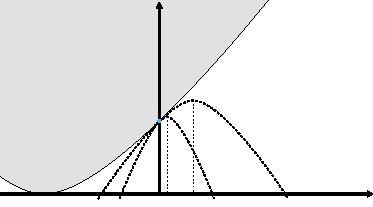
\includegraphics{part_2/chapter_9/figures/augmented_G.pdf}};
%		\draw[help lines] (-3,-2) grid (3,2);
		\node at (-2.5,1.5) {$G$};
		%\node at (-2,0.5) {\scriptsize $(h(x), f(x))$};
		\node[right] at (-0.5, 1.6) {\scriptsize $z = f(x)$};
		\node[left] at (3.2,-1.4) {\scriptsize $h(x) = \epsilon$}; 
		\node[right] at (1,1.3) {\scriptsize $v(\epsilon)$};
		\node[left] at (-0.4,-0.3) {\scriptsize $\epsilon_{\overline{\mu}}$};
		\node[right] at (0.2,-0.9) {\scriptsize $f + \overline{v}h + \mu_2 h^2$};		
		\node[right] at (0.65,-0.2) {\scriptsize $f + \overline{v}h + \mu_1 h^2$};
		\node[below] at (0.2,-1.5) {\scriptsize $\frac{-\overline{v}}{2\mu_1}$};	
		\node[below] at (-0.5,-1.5) {\scriptsize $\frac{-\overline{v}}{2\mu_2}$};	
	\end{tikzpicture}
	\caption{Geometric representation of augmented Lagrangians in the mapping $G = [h(x), f(x)]$} \label{fig:Fig2}
\end{figure}

Optimising the augmented Lagrangian function amounts to finding the curve $f + \overline{v}h + \mu h^2 = k$ in which $v(\epsilon) = k$. The expression for $k$ can be conveniently rewritten as $f = -\mu \left[ h + (\overline{v}/2\mu)\right]^2 + \left[k + (\overline{v}^2/4\mu)\right]$, exposing that $f$ is a parabola shifted by $h = -\overline{v}/2\mu$.


\subsection{Augmented Lagrangian method of multipliers}


We can employ an unconstrained optimisation method to solve the augmented Lagrangian function
$$ 
L_\mu(x,v) = f(x) + \sum_{i=1}^lv_ih_i(x) + \mu\sum_{i=1}^lh_i(x)^2,
$$
which amount to rely on strong duality and search for KKT points (or primal-dual pairs) $(\overline{x},\overline{v})$ by iteratively operating in the primal ($x$) and dual ($v$) spaces. In particular, the strategy consists of
\begin{enumerate}
\item \emph{Primal space:} optimise $L_\mu(x,v^k)$ using an unconstrained optimisation method
\item \emph{Dual space:} perform a dual variable update step retaining the optimality condition $\nabla_x L(x^{k+1},v^k) = \nabla_x L(x^{k+1},v^{k+1}) = 0$
\end{enumerate}

This strategy is akin to applying the subgradient method to solving the augmented Lagrangian dual. The update step for the dual variable is given by 
$$
\overline{v}^{k+1} = \overline{v}^k + 2\mu h(\overline{x}^{k+1}). 
$$

The motivation for the dual step update stems from the following observation:
%
\begin{enumerate}
\item $h(\overline{x}^k)$ is a subgradient of $L_\mu(x,v)$ at $\overline{x}^k$ for any $v$.
\item The step size is devised such that the optimality condition of the Lagrangian function is retained, i.e., $\nabla_x L(\overline{x}^k,\overline{v}^{k+1}) = 0$.
\end{enumerate}

Part 2 refers to the following:
%
\begin{align*}
\nabla_x L(\overline{x}^k,\overline{v}^{k+1}) & =  \nabla f(\overline{x}^k) + \sum_{i=1}^l\overline{v}^{k+1}_i\nabla h_i(\overline{x}^k) = 0 \\
& = \nabla f(\overline{x}^k)  + \sum_{i=1}^l(\overline{v}_i^{k} + 2\mu h_i(\overline{x}^k))\nabla h_i(\overline{x}^k) = 0 \\
& = \nabla f(\overline{x}^k) + \sum_{i=1}^l\overline{v}_i^{k}\nabla h_i(\overline{x}^k)\hspace{-1pt} + \sum_{i=1}^l2\mu h_i(\overline{x}^k)\nabla h_i(\overline{x}^k) = \nabla_x L_\mu(\overline{x}^k,\overline{v}^{k})=0.
\end{align*}

That is, by employing $\overline{v}^{k+1} = \overline{v}^k + 2\mu h(\overline{x}^{k+1})$ one can retain optimality in the dual variable space for the Lagrangian function from the optimality conditions of the penalised functions, which is a condition for $\overline{x}$ to be a KKT point. 

Algorithm \ref{Alg1} summarises the augmented Lagrangian method of multipliers (ALMM). 

\begin{algorithm}[H]
\caption{Augmented Lagrangian method of multipliers (ALMM)} \label{Alg1}
\begin{algorithmic}[1] %line numbering frequency.
\State {\bf initialise.} tolerance $\epsilon > 0,$ initial dual solution $v^0,$ iteration count $k = 0$  
\While {$|h(\overline{x}^k)| > \epsilon$} 
        \State $\overline{x}^{k+1} = \arg\min L_\mu(x,\overline{v}^k)$
        \State $\overline{v}^{k+1} = \overline{v}^{k} + 2\mu h(\overline{x}^{k+1})$
    \State $k = k+1$
\EndWhile
\State {\bf return} $x^k$.
\end{algorithmic}
\end{algorithm}

The method can be specialised such that $\mu$ is individualised for each constraint and updated proportionally to the observed infeasibility $h_i(x)$. Such a procedure is still guaranteed to converge, as the requirement in Theorem \ref{thm:conv_pen_method} that $\mu \rightarrow \infty$ is still trivially satisfied.

One important point about the augmented Lagrangian method of multipliers is that linear convergence is to be expected, due to the gradient-like step taken to find optimal dual variables. This is often the case with traditional Lagrangian duality based approaches.


\subsection{Alternating direction method of multipliers - ADMM}

ADMM is a distributed version of the augmented Lagrangian method of multipliers, and is more suited to large problems with a decomposable structure. 

Consider the problem $P$ to be of the following form:
%
\begin{align*}
(P) : \mini \ & f(x) + g(y) \\
\st &Ax + By = c.    
\end{align*}
%
We would like to be able to solve the problem separately for $x$ and $y$, which could, in principle be achieved using ALMM. However, the consideration of the penalty term prevents the problem from being completely separable. To see that, let
$$ 
\phi(x,y,v) = f(x) + g(y) + v^\top(c - Ax - By) + \mu(c - Ax - By)^2
$$
be the augmented Lagrangian function. One can notice that the penalty term $\mu(c - Ax - By)^2$ prevents the separation of the problem in terms of the $x$ and $y$ variables. However, separability can be recovered is one employs a coordinate descent approach in which three blocks are considered: $x$, $y$, and $v$. The ADMM is summarised in Algorithm \ref{Alg2}.

\begin{algorithm}[H]
\caption{ADMM} \label{Alg2}
\begin{algorithmic}[1] %line numbering frequency. 
\State {\bf initialise.} tolerance $\epsilon > 0,$ initial dual and primal solutions $v^0$ and $y^0,$ $k = 0$ 
\While {$|c - A\overline{x}^k - B\overline{y}^k| \text{ and } || y^{k+1} - y^{k} ||> \epsilon$} \label{stop_criteria}
        \State $\overline{x}^{k+1} = \arg\min \phi_\mu(x, \overline{y}^k ,\overline{v}^k)$ \label{x-step}
        \State $\overline{y}^{k+1} = \arg\min \phi_\mu(\overline{x}^{k+1}, y, \overline{v}^k)$  \label{y-step}
        \State $\overline{v}^{k+1} = \overline{v}^{k} + 2\mu (c - A\overline{x}^{k+1} - B\overline{y}^{k+1})$ \label{dual-step}
    \State $k = k+1$
\EndWhile
\State {\bf return} $(x^k, y^k)$.
\end{algorithmic}
\end{algorithm}

One important feature regarding ADMM is that the coordinate descent steps are taken in a cyclic order, not requiring more than one $(x,y)$ update step. Variants consider more than one of these steps, but no clear benefit in practice has been observed. Moreover, $\mu$ can be updated according to the amount of infeasibility observed at iteration $k$, but no generally good update rule is known. 

ADMM is particularly relevant as a method for (un)constrained problems in which it might expose a structure that can be exploited, such as having in some of the optimisation problems (in Lines \ref{x-step} and \ref{y-step} in Algorithm \ref{Alg2}) that might have solutions in closed forms.  


% Include examples from l1-regression and LP/QP.

%Consider the following example, arising from applications of $l_1$-regularisation. Let $f: \reals^n \mapsto \reals$ convex and $X$ a closed convex set. $P$ is defined as
%$$
%(P) : \mini_{x \in X} \ f(x) + \gamma||x||_1, 
%$$
%
%In this case, the augmented Lagrangian function is given by
%$$
%\phi(x,z,v) = f(x) + \gamma||z||_1 + v^\top(x-z) + \frac{\mu}{2}(x-z)^2
%$$
%
%The ADMM steps are given by
%\begin{itemize}	
%\item $x_{k+1} = \arg\min_{x \in X} \braces{f(x) + v_{k}^\top x + \frac{\mu}{2}(x - z_k)^2}$
%\item $z_{k+1} = \arg\min_{z \in {\bf R}^n} \braces{\gamma||z|| - v_{k}^\top z + \frac{\mu}{2}(x_{k+1} - z)^2}$
%\item $v_{k+1} = v_k + \mu (x_{k+1} - z_{k+1})$.
%\end{itemize}
%
%The $z$-step has a closed form using the \emph{shrinkage operation}: 
%\begin{align*}
%	z^{k+1}_i = \begin{cases} x^{k+1}_i + \frac{v^k - \gamma}{\mu}, \text{ if } x^{k+1}_i + \frac{v^k}{\mu} > \frac{\gamma}{\mu} \\
% 							  0,  \text{ if } \left|x^{k+1}_i + \frac{v^k}{\mu} \right| \leq \frac{\gamma}{\mu} \\
% 							  x^{k+1}_i + \frac{v^k + \gamma}{\mu}, 	 \text{ if } x^{k+1}_i + \frac{v^k}{\mu} < \frac{\gamma}{\mu}	
% 				\end{cases}
%\end{align*}
%making the optimisation of $P$ \emph{efficiently separable}. 
%

%% Discuss ADMM in more detail, giving details of how residuals are calculated and a demonstration on how the shrinkage operation is indeed optimal. 
